\documentclass[oneside, 10pt, notitlepage]{book}
	
\usepackage{../_mypackages/monographpreamble}
\usepackage{../_mypackages/commands}

\title{Special Relativity} % \MyTitle
\author{Bruno Murino} % \MyAuthor
\date{\today} % \MyDate

\usepackage{../_mypackages/monographstyle}

\graphicspath{ {figures/} }

%--------------------------------------------------------------------------------------------------

\begin{document}
\chapter{Lista XIII}

\section*{Ex. 1)}

Let \(A_{\mu\nu}\) be a tensor. We define its symmetric part as
\begin{equation}
    A_{(\mu\nu)} = \hlf \lr{A_{\mu\nu}+A_{\nu\mu}}
\end{equation}
and its anti symmetric part as
\begin{equation}
    A_{[\mu\nu]} = \hlf \lr{A_{\mu\nu}-A_{\nu\mu}}
\end{equation}

\subsection*{(a)}
Lets do
\begin{equation}
    A_{(\mu\nu)}+A_{[\mu\nu]} = \hlf \lr{A_{\mu\nu}+A_{\nu\mu}}+\hlf \lr{A_{\mu\nu}-A_{\nu\mu}} = \hlf \lr{2 A_{\mu\nu}} = A_{\mu\nu}
\end{equation}

\subsection*{(b)}

Lets compute \(A_{(\mu\nu)}B^{\mu\nu}\)
\begin{equation}
    A_{(\mu\nu)}B^{\mu\nu} = \hlf \lr{A_{\mu\nu}+A_{\nu\mu}}B^{\mu\nu} = \hlf \lr{A_{\mu\nu}B^{\mu\nu} + A_{\nu\mu}B^{\mu\nu}}
\end{equation}
Now \(A_{(\mu\nu)}B^{(\mu\nu)}\)
\begin{equation}
\begin{split}
    A_{(\mu\nu)}B^{(\mu\nu)} &= \hlf \lr{A_{\mu\nu}+A_{\nu\mu}}\hlf \lr{B_{\mu\nu}+B_{\nu\mu}} \\
    &=\frac{1}{4}\lr{A_{\mu\nu}B^{\mu\nu} + A_{\mu\nu}B^{\nu\mu} + A_{\nu\mu}B^{\mu\nu}+A_{\nu\mu}B^{\nu\mu}}\\
    &= \hlf \lr{A_{\mu\nu}B^{\mu\nu} + A_{\nu\mu}B^{\mu\nu}}
\end{split}
\end{equation}
since repeated indices can be relabelled without loss of meaning (dummy indices). And finally \(A_{\mu\nu}B^{(\mu\nu)}\)
\begin{equation}
\begin{split}
    A_{\mu\nu}B^{(\mu\nu)} &= A_{\mu\nu}\hlf \lr{B^{\mu\nu}+B^{\nu\mu}} \\
    &= \hlf \lr{A_{\mu\nu} B^{\mu\nu} + A_{\mu\nu}B^{\nu\mu}}\\
    &= \hlf \lr{A_{\mu\nu} B^{\mu\nu} + A_{\nu\mu}B^{\mu\nu}}
\end{split}
\end{equation}
Comparing the results we can see that \(A_{(\mu\nu)}B^{\mu\nu}=A_{(\mu\nu)}B^{(\mu\nu)}=A_{\mu\nu}B^{(\mu\nu)}\).

\subsection*{(c)}

Lets compute \(A_{\mu\nu}B^{[\mu\nu]}\)
\begin{equation}
\begin{split}
    A_{(\mu\nu)}B^{[\mu\nu]} &= \hlf \lr{A_{\mu\nu}+A_{\nu\mu}} \hlf \lr{B^{\mu\nu}-B^{\nu\mu}} \\
    &= \frac{1}{4} \lr{A_{\mu\nu}B^{\mu\nu} - A_{\mu\nu}B^{\nu\mu} + A_{\nu\mu}B^{\mu\nu} - A_{\nu\mu}B^{\nu\mu}} \\
    &= 0
\end{split}
\end{equation}

\subsection*{(d)}

Its easy to see that the results are analogous if we let \((\mu\nu)\leftrightarrow [\mu\nu]\).

\section*{Ex. 2)}


\section*{Ex. 3)}

A frame \(S'\) is moving away with respect to the frame \(S\) with speed \(u\) along the \(x\)-axis. Both frames measure the speed of a particle along the \(x\)-axis: \(S\) finds \(v\) while \(S'\) finds \(v'\). Then, Einstein velocity addition implies that
\begin{equation}\label{eq:einsvel}
    v' = \frac{v-u}{1-\frac{vu}{c^2}} \qq{or} \frac{v'}{c^2} = \frac{v-u}{c^2 - vu}
\end{equation}
If the frame is moving with speed \(-u\), we just need to plug this into \eqref{eq:einsvel}, thus
\begin{equation}\label{eq:einsvelminus}
    \frac{v'}{c^2} = \frac{v+u}{c^2+vu}
\end{equation}

\subsection*{(a)}

With respect to a frame at rest \(S\), if two objects with mass \(m_1\) and \(m_2\) are moving along the \(x\)-axis with speed \(v_1\) and \(v_2\), with \(v_1 > v_2\), they collide, and after the collision, their respective speeds are \(v_3\) and \(v_4\). If there's a frame \(S'\) moving along the \(x\)-axis with speed \(-u\), then the correct speeds seen by \(S'\) are given by \eqref{eq:einsvelminus}, thus
\begin{equation}
    \frac{v'_i}{c^2} = \frac{v_i + u}{c^2 + v_i u} \qq{for} i = 1,2,3,4 
\end{equation}

\subsection*{(b)}
The classical conservation of momentum is
\begin{equation}\label{eq:momconsclass}
    m_1 v_1 + m_2 v_2 = m_1 v_3 + m_2 v_4 \qq{thus} m_1 \lr{\frac{v_1}{c^2}-\frac{v_3}{c^2}} = m_2 \lr{\frac{v_4}{c^2}-\frac{v_2}{c^2}}
\end{equation}
So, with respect to \(S'\) it will read
\begin{equation}\label{eq:momconsprimeclass}
    m_1 v'_1 + m_2 v'_2 = m_1 v'_3 + m_2 v'_4 \qq{thus} m_1 \lr{\frac{v'_1}{c^2}-\frac{v'_3}{c^2}} = m_2 \lr{\frac{v'_4}{c^2}-\frac{v'_2}{c^2}}
\end{equation}
Lets compute \(\frac{v'_1}{c^2}-\frac{v'_3}{c^2}\)
\begin{equation}
\begin{split}
    \frac{v'_1}{c^2}-\frac{v'_3}{c^2} &=  \frac{v_1 + u}{c^2 + v_1 u} - \frac{v_3 + u}{c^2 + v_3 u} \\ 
    &= \frac{(v_1 + u)(c^2 + v_3 u) - (v_3 + u)(c^2 + v_1 u)}{(c^2 + v_1 u)(c^2 + v_3 u)} \\
    &= \frac{v_1 c^2 + uc^2 + uv_1v_3 + u^2 v_3 - (v_3c^2 + uc^2 + uv_1v_3 + u^2 v_1)}{(c^2 + v_1 u)(c^2 + v_3 u)} \\
    &= \frac{c^2(v_1 - v_3) - u^2(v_1-v_3)}{(c^2 + v_1 u)(c^2 + v_3 u)} \\
    &= \frac{(v_1-v_3)(c^2 - u^2)}{(c^2 + v_1 u)(c^2 + v_3 u)}
\end{split}
\end{equation}
And analogous for \(\frac{v'_4}{c^2}-\frac{v'_2}{c^2}\). Plugging this result on \eqref{eq:momconsprimeclass}, and using \eqref{eq:momconsclass}, we find that the following must be satisfied
\begin{equation}
    (c^2 + v_1 u)(c^2 + v_3 u) = (c^2 + v_4 u)(c^2 + v_2 u)
\end{equation}
This equation can be interpreted as a constrain on \(u\), meaning that given \(v_1\), \(v_2\), \(v_3\) and \(v_4\), \(u\) would be fully determined, what doesn't make any sense, since we can have a moving frame with any speed we want. If we had found an identity, like \(0=0\), we could conclude that everything was ok, but this was not the case.

The correct momentum conservation equation is
\begin{equation}\label{eq:momconsrel}
    \gamma_1 m_1 v_1 + \gamma_2 m_2 v_2 = \gamma_3 m_1 v_3 + \gamma_4 m_2 v_4 \qq{thus} m_1 \lr{\frac{\gamma_1 v_1}{c}-\frac{\gamma_3 v_3}{c}} = m_2 \lr{\frac{\gamma_4 v_4}{c}-\frac{\gamma_2 v_2}{c}}
\end{equation}
and, with respect to \(S'\), it will read
\begin{equation}\label{eq:momconsprimerel}
    \gamma'_1 m_1 v'_1 + \gamma'_2m_2 v'_2 = \gamma'_3m_1 v'_3 + \gamma'_4m_2 v'_4 \qq{thus} m_1 \lr{\frac{\gamma'_1v'_1}{c}-\frac{\gamma'_3v'_3}{c}} = m_2 \lr{\frac{\gamma'_4v'_4}{c}-\frac{\gamma'_2v'_2}{c}}
\end{equation}
where \(\gamma_i = \gamma (v_i)\), and analogous for \(\gamma'_i\).

Lets compute \(\frac{\gamma'_1v'_1}{c}\)
\begin{equation}
\begin{split}
    \frac{\gamma'_1v'_1}{c} &= \frac{v'_1}{\sqrt{c^2-v_1^{\prime2}}}\\
    &= c^2\lr{\frac{v_1 + u}{c^2 + v_1 u}}\frac{1}{\sqrt{c^2 -c^4 \lr{\frac{v_1 + u}{c^2 + v_1 u}}^2 }} \\
    &= \frac{c(v_1 + u)}{\sqrt{\lr{c^2 + v_1 u}^2 - c^2\lr{v_1 + u}^2}} \\
    &= \frac{c(v_1 + u)}{\sqrt{c^4 + 2 v_1 u c^2 + v_1^2 u^2 - \lr{c^2v_1^2 + 2 v_1 uc^2 + u^2c^2}}} \\
    &= \frac{(v_1 + u)}{\sqrt{c^2 -u^2 - v_1^2\lr{1-\frac{u^2}{c^2}}}} \\
    &= \frac{(v_1 + u)}{\sqrt{c^2 -u^2 - \frac{v_1^2}{c^2}\lr{c^2-u^2}}} \\
    &= \frac{(v_1 + u)}{\sqrt{\lr{c^2 -u^2}\lr{1- \frac{v_1^2}{c^2} } }} \\
    &= \frac{\gamma_1(v_1 + u)}{\sqrt{\lr{c^2 -u^2}} } \\
    &= \frac{\gamma_1 v_1 + \gamma_1 u}{\sqrt{\lr{c^2 -u^2}}}
\end{split}
\end{equation}
So \eqref{eq:momconsprimerel} becomes
\begin{equation}
    m_1 \lr{\frac{\gamma_1 v_1 + \gamma_1 u}{\sqrt{\lr{c^2 -u^2}}}-\frac{\gamma_3 v_3 + \gamma_3 u}{\sqrt{\lr{c^2 -u^2}}}} = m_2 \lr{\frac{\gamma_4 v_4 + \gamma_4 u}{\sqrt{\lr{c^2 -u^2}}}-\frac{\gamma_2 v_2 + \gamma_2 u}{\sqrt{\lr{c^2 -u^2}}}}
\end{equation}
thus
\begin{equation}
    m_1 \lr{\gamma_1 v_1 + \gamma_1 u-\gamma_3 v_3 - \gamma_3 u} = m_2 \lr{\gamma_4 v_4 + \gamma_4 u-\gamma_2 v_2 - \gamma_2 u}
\end{equation}
then
\begin{equation}
    m_1\lr{\gamma_1 v_1 -\gamma_3 v_3} + m_1 u \lr{\gamma_1-\gamma_3} = m_2\lr{\gamma_4 v_4 -\gamma_2 v_2} + m_2 u \lr{\gamma_4-\gamma_2} 
\end{equation}
and due to \eqref{eq:momconsrel} we find
\begin{equation}
    m_1 \lr{\gamma_1-\gamma_3} = m_2 \lr{\gamma_4-\gamma_2} 
\end{equation}
Hold on to this result. Lets compute what should the energy conservation equation be on both frames
\begin{equation}
    \gamma_1 m_1 c^2 +\gamma_2 m_2 c^2 = \gamma_3 m_1 c^2 +\gamma_4 m_2 c^2 \qq{for \(S\)}
\end{equation}
and
\begin{equation}
    \gamma'_1 m_1 c^2 +\gamma'_2 m_2 c^2 = \gamma'_3 m_1 c^2 +\gamma'_4 m_2 c^2 \qq{for \(S'\)}
\end{equation}
So, from the energy conservation on \(S\), we already can see that it can be written as
\begin{equation}
    m_1 \lr{\gamma_1-\gamma_3} = m_2 \lr{\gamma_4-\gamma_2} 
\end{equation}
which is exactly what came out from both equations for momentum conservation! So far everything is consistent!


\section*{Ex. 4)}

First, the 4-momentum definition is
\begin{equation}
    p^{\mu} = \lr{E/c,p_x,p_y,p_z}
\end{equation}
and the Lorentz transformation is given by
\begin{subequations}
    \begin{align}[left = \empheqlbrace\,]
    & E'/c = \gamma(v)\lr{E/c - \beta p_x} \\
	& p_x = \gamma(v)\lr{p_x - \beta E/c} \\
	& p'_y= p_y \\
	& p'_z = p_z
    \end{align}
\end{subequations}

\subsection*{(a)}
If we have
\begin{equation}
    p^{\mu} = \lr{\frac{h\nu}{c},\frac{h\nu}{c},0,0} \qq{with respect to \(S\)}
\end{equation}
and
\begin{equation}
    p'^{\mu} = \lr{\frac{h\nu'}{c}, \frac{h\nu'}{c},0,0} \qq{with respect to \(S'\)}
\end{equation}
then, thanks to the Lorentz transformation for the energy, we have
\begin{equation}
    \frac{h\nu'}{c} = \gamma \lr{ \frac{h\nu}{c} - \beta \frac{h\nu}{c}} = h \nu \gamma \lr{1-\beta}
\end{equation}
then
\begin{equation}
    \frac{\nu'}{\nu} = \gamma (1-\beta) = \lr{\frac{1+\beta}{1-\beta}}^{1/2}
\end{equation}
which is the same as the Doppler effect formula.

\subsection*{(b)}
If we have
\begin{equation}
    p^{\mu} = \lr{\frac{h\nu}{c},\frac{h\nu\cos \alpha}{c},\frac{h\nu\sin \alpha}{c},0} \qq{with respect to \(S\)}
\end{equation}
and
\begin{equation}
    p'^{\mu} = \lr{\frac{h\nu'}{c},\frac{h\nu'\cos \alpha'}{c},\frac{h\nu'\sin \alpha'}{c},0} \qq{with respect to \(S'\)}
\end{equation}
then, thanks to the Lorentz transformation for the energy, we have
\begin{equation}
    \frac{h\nu'}{c} = \gamma \lr{\frac{h\nu}{c} - \beta\frac{h\nu\cos \alpha}{c}} = h\nu \gamma \lr{1-\beta \cos\alpha}
\end{equation}
then
\begin{equation}
    \frac{\nu'}{\nu} = \gamma \lr{1-\beta \cos\alpha}
\end{equation}
and thanks to the Lorentz transformation for \(p_x\), we have
\begin{equation}
    \frac{h\nu'\cos \alpha'}{c} = \gamma \lr{\frac{h\nu\cos \alpha}{c} - \beta \frac{h\nu}{c}}
\end{equation}
which implies
\begin{equation}
    \frac{\nu'}{\nu} \cos \alpha' = \gamma \lr{\cos \alpha - \beta}
\end{equation}
which further impliespip install pyinstaller
\begin{equation}\label{eq:cosprime}
    \cos \alpha' = \frac{\cos \alpha -\beta}{1-\beta \cos \alpha}
\end{equation}
Also, thanks to the Lorentz transformation for \(p_y\), we have
\begin{equation}
    \frac{h\nu\sin \alpha}{c} = \frac{h\nu'\sin \alpha'}{c}
\end{equation}
thus
\begin{equation}
    \sin \alpha' = \frac{\nu}{\nu'}\sin \alpha
\end{equation}
which leads to
\begin{equation}\label{eq:sinprime}
    \sin \alpha' = \frac{\sin \alpha}{\gamma \lr{1-\beta \cos\alpha}}
\end{equation}

\section*{Ex. 5) Solution by Martim Zurita.}

\begin{figure}[H]
    \label{fig:L13_5}
    \centering
    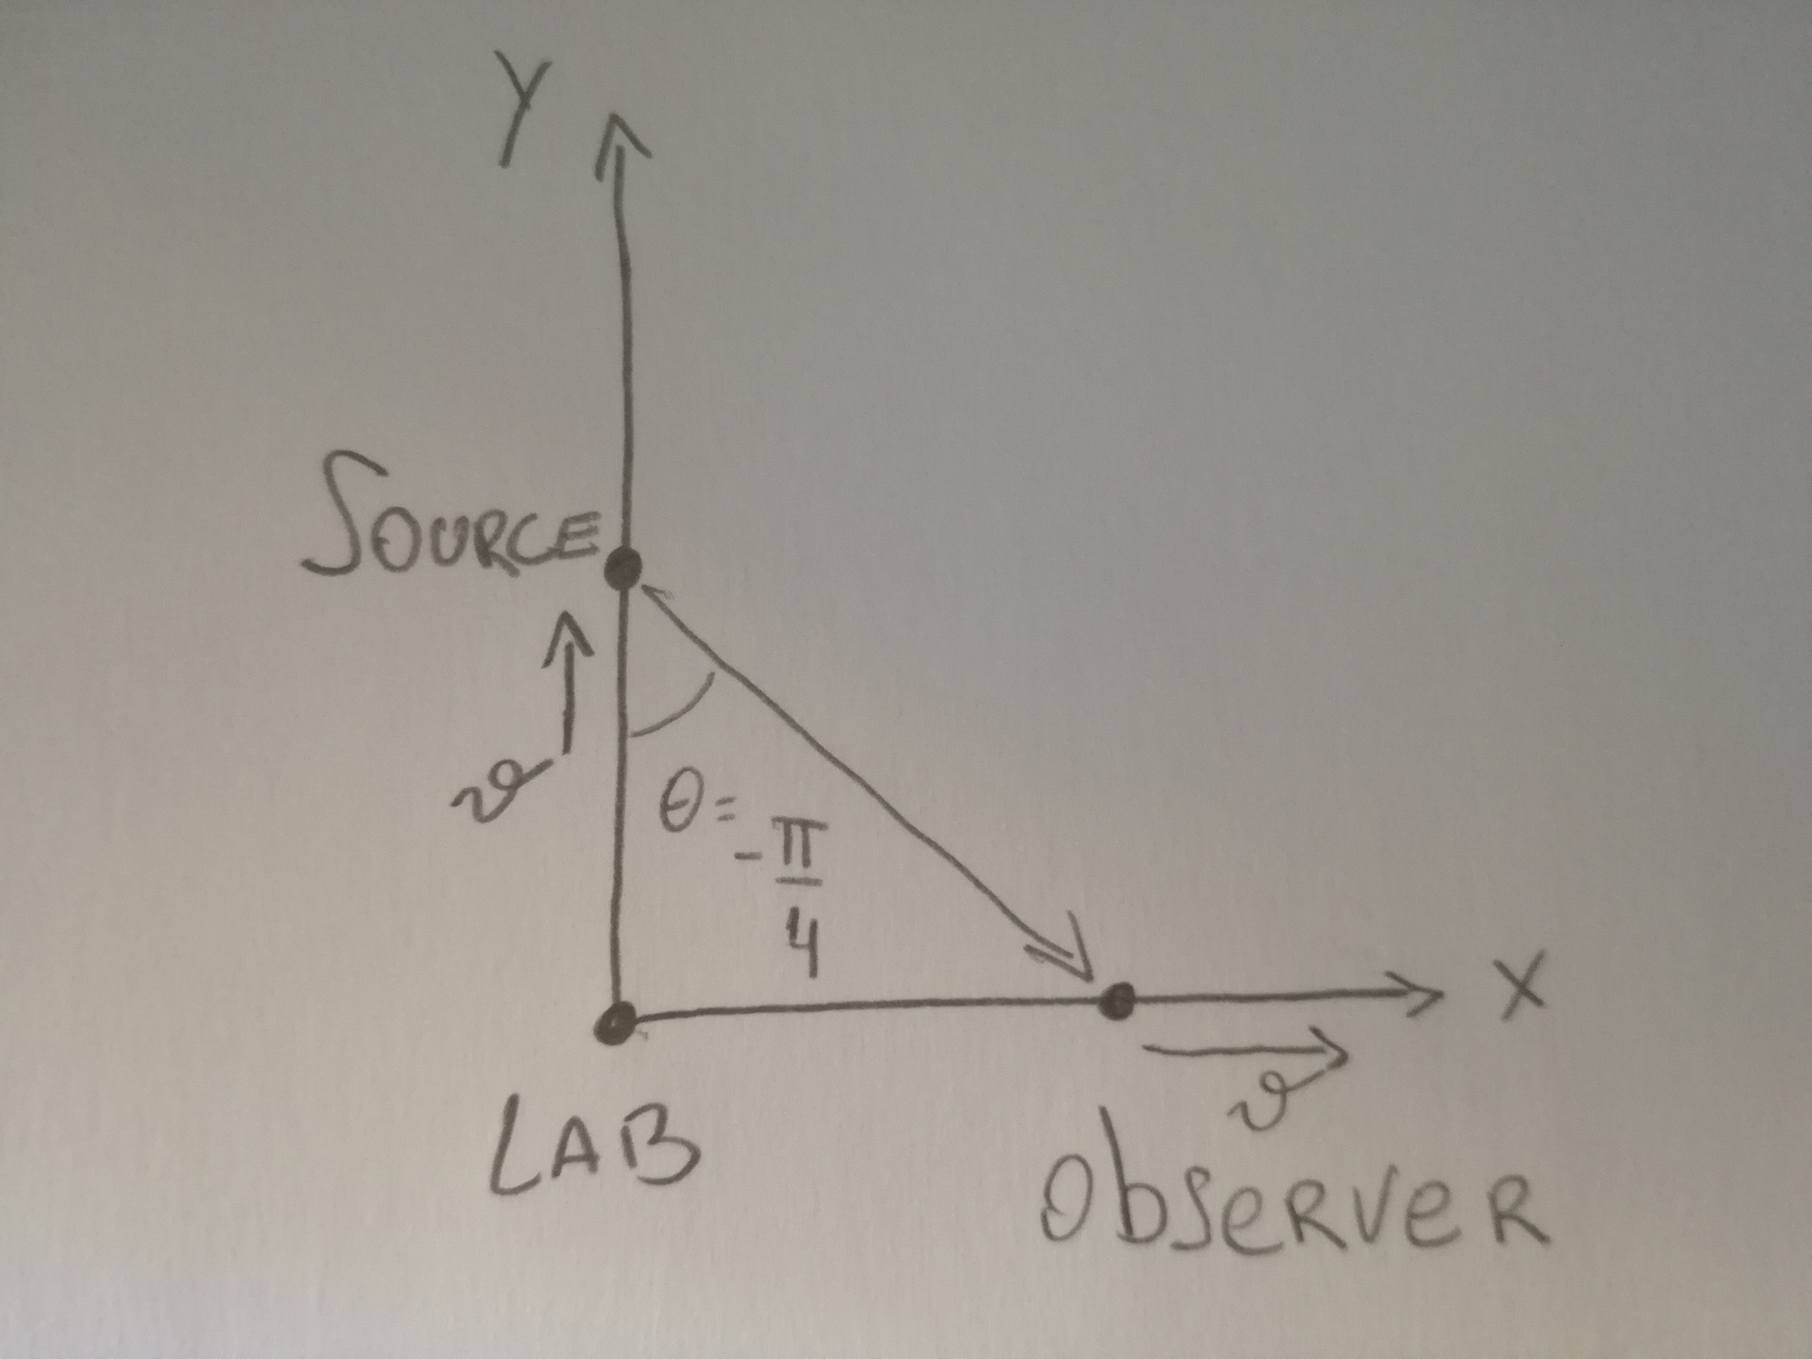
\includegraphics[width=0.5\textwidth]{L13_5}
    \caption{Diagram of problem 5.}
\end{figure}  

We have the laboratory frame \(S\), the source frame \(S_s\) and the observer frame \(S_o\). The four-momentum of the emitted photon can be written as 
\begin{equation}
    p^{\mu} = \lr{\frac{h \nu}{c},\frac{h \nu\cos\theta}{c}, \frac{h \nu\sin\theta}{c},0 } \qq{with respect to the lab}
\end{equation}
\begin{equation}
    p_s^{\mu} = \lr{\frac{h \nu_s}{c},\frac{h \nu_s\cos\theta_s}{c}, \frac{h \nu_s\sin\theta_s}{c},0 }  \qq{with respect to the source}
\end{equation}
\begin{equation}
    p_o^{\mu} = \lr{\frac{h \nu_o}{c},\frac{h \nu_o\cos\theta_o}{c}, \frac{h \nu\sin\theta_o}{c},0 }  \qq{with respect to the observer}
\end{equation}

Figure \ref{fig:L13_5} shows a diagram of the problem.

Since the source moves with speed \(v_s\) along the \(y\)-axis with respect to the lab, the Lorentz transformation and its inverse for the frequency between the source frame and the lab frame is
\begin{equation}\label{eq:labsourcedop}
\begin{split}
    \frac{E_s}{c} = \gamma_s \lr{\frac{E}{c}-\beta_s p_y} \qq{thus} \nu_s = \gamma_s \nu \lr{1-\beta_s \sin \theta} \\
    \frac{E}{c} = \gamma_s \lr{\frac{E_s}{c}+\beta_s p_{sy}} \qq{thus} \nu = \gamma_s \nu_s \lr{1+\beta_s \sin \theta_s}
\end{split}
\end{equation}
where \(\gamma_s\) is the Lorentz factor with \(v = \pm v_s\), and \(\beta_s = v_s/c\). These relations represent the Doppler effect between the lab and the source. If we multiply the equations on \eqref{eq:labsourcedop}, we find
\begin{equation}
    \nu_s \nu = \gamma_s^2 \nu_s \nu \lr{1-\beta_s \sin\theta}\lr{1+\beta_s\sin\theta_s}
\end{equation}
thus
\begin{equation}\label{eq:thetalabsource}
    \frac{1}{\gamma_s^2\lr{1-\beta_s \sin\theta}} = 1+\beta_s\sin\theta_s
\end{equation}
which implicitly gives us the relation between \(\theta_s\) and \(\theta\).

On the other hand, we can also find, again through the Lorentz transformations, the doppler effect between the lab and the observer, which moves along the \(x\)-axis with speed \(v_o\)
\begin{equation}
    \nu_o = \gamma_o \nu \lr{1-\beta_o \cos\theta}
\end{equation}  
We can now plug \(\nu\) from the second equation of \eqref{eq:labsourcedop} to find the relation between \(\nu_o\) and \(\nu_s\)
\begin{equation}
    \nu_o = \gamma_o \ssb{\gamma_s \nu_s \lr{1+\beta_s\sin\theta_s}}\lr{1-\beta_o\cos\theta} = \gamma_o\gamma_s \nu_s \lr{1+\beta_s\sin\theta_s}\lr{1-\beta_o \cos\theta}
\end{equation}
We can then plug \eqref{eq:thetalabsource} to find 
\begin{equation}
    \nu_o = \gamma_o\gamma_s \nu_s \lr{\frac{1}{\gamma_s^2\lr{1-\beta_s \sin\theta}}}\lr{1-\beta_o \cos\theta}
\end{equation}
thus
\begin{equation}
    \frac{\nu_o}{\nu_s} = \frac{\gamma_o}{\gamma_s} \lr{\frac{1-\beta_o \cos\theta}{1-\beta_s \sin\theta}}
\end{equation}
If the speed of the source and the observer have the same magnitude, and depart from the lab at the same time, implying \(\theta=-\pi/4\), we find that 
\begin{equation}
    \frac{\nu_o}{\nu_s} = \frac{1-\beta \frac{1}{\sqrt{2}}}{1+\beta \frac{1}{\sqrt{2}}} = \frac{\sqrt{2}-\beta}{\sqrt{2}+\beta}
\end{equation}

\section*{Ex. 6)}

From a mirror perspective, the incident and reflected light wave have the same frequency \(\nu\), and make the same angle \(\alpha\) with the normal. From the perspective of a moving frame (with respect to the mirror), the incident light wave has frequency \(\nu_1\) and makes \(\theta\) angles with the normal while the reflected light wave has frequency \(\nu_2\) and makes \(\phi\) angles with the normal.

\begin{figure}[H]
    \centering
    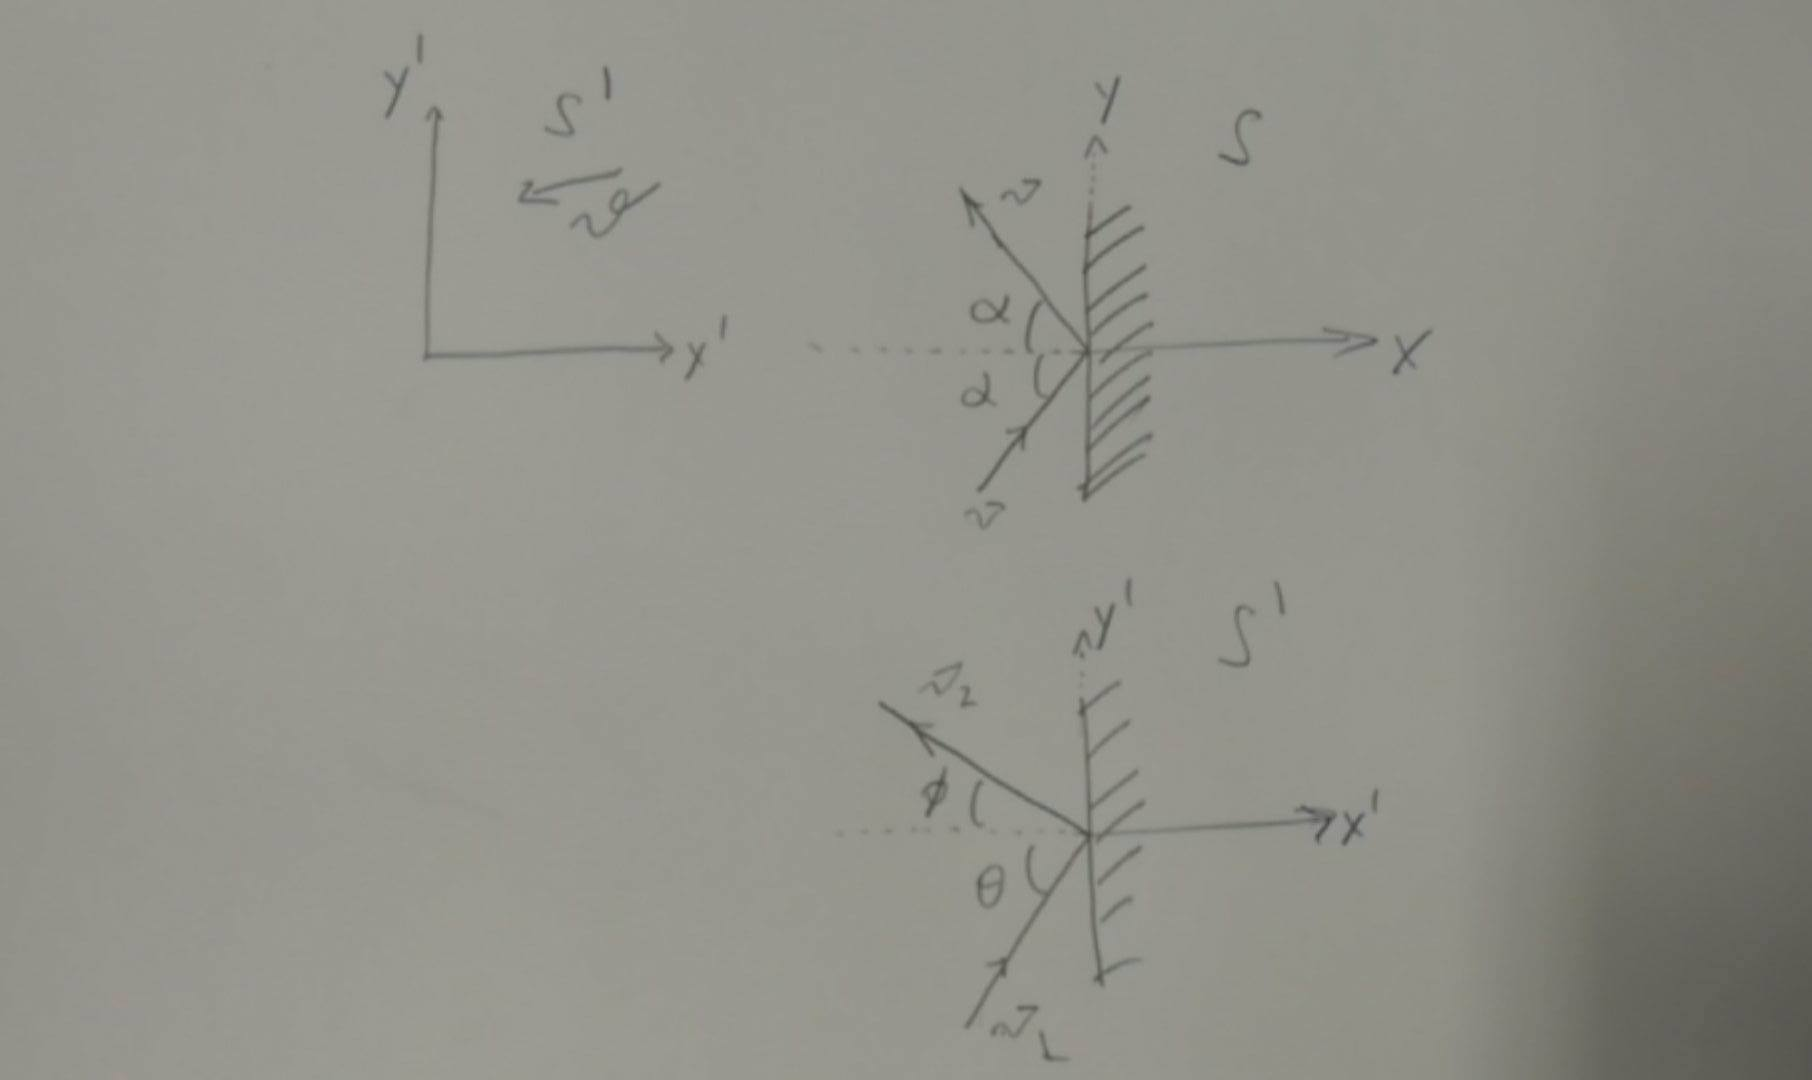
\includegraphics[width = 0.7 \textwidth]{L13_6}
    \caption{Diagram of problem 6.}
    \label{fig:L13_6}
\end{figure}

For the incident wave, we have
\begin{equation}
    p^{\mu} = \lr{\frac{h\nu}{c},\frac{h\nu\cos \alpha}{c},\frac{h\nu\sin \alpha}{c},0 } \qq{with respect to the mirror}
\end{equation}
and
\begin{equation}
    p'^{\mu} = \lr{\frac{h\nu_1}{c},\frac{h\nu_1\cos \theta}{c},\frac{h\nu_1\sin \theta}{c},0 } \qq{with respect to the moving frame}
\end{equation}
while for the reflected wave, we have
\begin{equation}
    p^{\mu} = \lr{\frac{h\nu}{c},-\frac{h\nu\cos \alpha}{c},\frac{h\nu\sin \alpha}{c},0 } \qq{with respect to the mirror}
\end{equation}
and
\begin{equation}
    p'^{\mu} = \lr{\frac{h\nu_2}{c},-\frac{h\nu_2\cos \phi}{c},\frac{h\nu_2sin \phi}{c},0 } \qq{with respect to the moving frame}
\end{equation}
It was shown before that
\begin{equation}
    \cos \alpha'= \frac{\cos \alpha - \beta}{1 - \beta \cos \alpha}
\end{equation}
Regarding the incident wave, \(\alpha' = \theta\)
\begin{equation}
    \cos \theta = \frac{\cos \alpha - \beta}{1 - \beta \cos \alpha}
\end{equation}
and regarding the reflected wave, the minus sign on \(p_x\) implies the change \(\beta \leftarrow -\beta\), thus
\begin{equation}
    \cos\phi = \frac{\cos \alpha + \beta}{1 + \beta \cos \alpha}
\end{equation}

Since 
\begin{equation}
    \tan^2 \frac{\theta}{2} = \frac{1-\cos \theta}{1+\cos \theta}
\end{equation}
by plugging \(\cos\theta\) we find that
\begin{equation}
    \tan^2 \frac{\theta}{2} = \frac{1+\beta}{1-\beta} \tan^2 \frac{\alpha}{2}
\end{equation}
Analogous for \(\phi\), we find
\begin{equation}
    \tan^2\frac{\phi}{2} = \frac{1-\beta}{1+\beta} \tan^2 \frac{\alpha}{2}
\end{equation}
which implies
\begin{equation}
    \frac{\tan^2 \frac{\theta}{2}}{\tan^2\frac{\phi}{2}} = \lr{\frac{1+\beta}{1-\beta}}
\end{equation}

\subsection*{(b)}

The Lorentz transformation for the Energy gives
\begin{equation}
    \frac{h\nu_1}{c} = \gamma \lr{\frac{h\nu}{c} - \beta \frac{h\nu \cos \alpha}{c}} \qq{for the incident wave}
\end{equation}
and
\begin{equation}
    \frac{h\nu_2}{c} = \gamma \lr{\frac{h\nu}{c} + \beta \frac{h\nu \cos \alpha}{c}} \qq{for the reflected wave}
\end{equation}
Then, taking one over the other, we find
\begin{equation}\label{eq:nu1nu2}
    \frac{\nu_2}{\nu_1} = \frac{1+\beta \cos \alpha}{1-\beta \cos \alpha}
\end{equation}
But, due to \eqref{eq:cosprime} and \eqref{eq:sinprime}, we know that
\begin{equation}
    1-\beta \cos \alpha = \frac{\sin \alpha}{\gamma \sin \theta} \qq{and} 1+\beta \cos \alpha = \frac{\cos \alpha + \beta}{\cos \phi}
\end{equation}
Plugging this onto \eqref{eq:nu1nu2}, we find that
\begin{equation}
    \frac{\nu_2}{\nu_1} = \frac{\sin \theta}{\cos \phi} \ssb{\frac{\gamma \lr{\cos \alpha + \beta}}{\sin \alpha}}
\end{equation}



% \backmatter
% \printbib
\end{document}
	